%!TEX root = ../thesis.tex

\chapter{Iron Flotation Layers in Mercury}
\label{chap:floatationlayers}
A model to explain the strength of Mercury's magnetic field was proposed by \citet{smith2012} using gravitational data from the MESSENGER probe. To construct an interior model of Mercury, they synthesised observations of Mercury's gravitational moments, as well as moment of inertia measurements derived from Earth based observations of Mercury's rotational state. Their inversions revealed the possibility of a deep, dense layer in Mercury's mantle. They proposed that this layer is composed of FeS, which solidified and floated on Mercury's bulk core due to the unique way in which Mercury's core may be freezing. They proposed this layer would attenuate the dynamo generated magnetic field via the screening effect before it reached the surface, producing Mercury's weak observed magnetic field. In this section we will implement this deep, dense, electrically conducting mantle in a numerical dynamo model to learn whether it can help explain Mercury's weak observed magnetic field.

\section{Gravity }
Gravitational measurements provide an important tool for learning about the structure of planets. Because the gravity field is a superposition of the field from all the material in the planet, it is sensitive to the deep interior of the planet. While gravitational inversions are not unique, they can be combined with other measurements to help constrain interior structure models.

\subsection{Introduction to Gravity}
Because the gravitational force is irrotational ($\nabla \times\mbf{g}=0$, where $\mbf{g}$ is the acceleration due to gravity) we can write it as the gradient of a scalar potential
\begin{equation}
\mbf{g}=-\nabla\Phi.
\end{equation}
In section \ref{sec:representations} we showed that this means $\Phi$ is a solution to Laplace's equation, which allows us to expand the angular part in a spherical harmonic expansion. The gravitational spherical harmonic expansion is usually written as 

\begin{equation}
\Phi\left(\mbf{r}\right)=-\frac{GM}{r}\left\{1-\sum_{l=1}^{\infty}\sum_{m=0}^{l}\left(\frac{a}{r}\right)^{l}P_{l}^{m}\left(\cos\theta\right)\left[C_{l}^{m}\cos\left(m\theta\right)+S_{l}^{m}\sin\left(m\theta\right)\right]\right\}
\label{eq:gravityexpansion}
\end{equation}
where $G$ is the gravitational constant, $M$ is the mass of the planet, $a$ is the planet's equatorial radius, and $P_l^m$ is a Schmidt normalised associated Legendre polynomial. Here $C_l^m$ and $S_l^m$ are known as the gravitational moments, which can be computed by
\begin{equation}
\left\{
\begin{array}{c}
C_l^m\\
S_l^m
\end{array}
\right\}=-\frac{1}{M}\int_{V}\rho\left(r,\theta,\phi\right) \left(\frac{r}{a}\right)^l P_{l}^{m}\left(\cos\theta\right)\left\{
\begin{array}{c}
\cos m\theta\\
\sin m \theta
\end{array}
\right\}
dV.
\label{eq:gravitycoefficients}
\end{equation}
Importantly these are sensitive to the density distribution of the planet. We see that in equation \ref{eq:gravitycoefficients} the density $\rho$ is weighted by $\left(r/a\right)^l$. This means that the shallower layers of the planet (where $r/a\approx 1$) have a greater effect on the higher harmonics than the deeper layers.

There are two other important notes we will make concerning equation \ref{eq:gravityexpansion}. First, if we pick the origin of our coordinate system to coincide with the centre of mass of our body, the components with $l=1$ vanish (we will do this from now on). Second, the gravitational harmonics of degree 2 can be related to the moments of inertia of the planet. Specifically, if $A$, $B$, and $C$ are the moments of inertia around the three principal axes of the planet we can write
%Specifically, if $I_{jk}$ denotes the components of the moment of inertia tensor in cartesian coordinates, the diagonal elements $I_{11}, I_{22}, I_{33}$ represent the moments of inertia around the three principal axes $A$, $B$, $C$ respectively. We can also relate the gravitational moments to the moments of inertia as
\begin{align}
C_2^0&=\frac{A+B-2C}{2a^2 M} \label{eq:C20}\\
%C_2^1&=\frac{I_{13}}{a^2 M}=\frac{I_{31}}{a^2 M} \\
%S_2^1&=\frac{I_{23}}{a^2 M}=\frac{I_{32}}{a^2 M} \\
C_2^2&=\frac{1}{4a^2 M} \left(B-A\right). \label{eq:C22}
%S_2^2&=\frac{1}{2 a^2 M} I_{12} = \frac{1}{2 a^2 M} I_{21}
\end{align}
For further details regarding this derivation see \citet{kaula1968}.

\section{Physical Librations of Mercury}
Because Mercury orbits so closely to the sun, it experiences gravitational torques associated with its permanent deformation. This causes a longitudinal libration in Mercury's spin which can be related to the moments of inertia
\begin{equation}
\phi_{0}=\frac{3}{2}\left(\frac{B-A}{C}\right)\left(1-11e^2+\frac{959}{48}e^4+\ldots\right)
\label{eq:librationamp}
\end{equation}
where $\phi_{0}$ is the amplitude of the libration, and $A$, $B$ and $C$ are the moments of inertia around the principle axes \citep{peale1972}. As we discussed in chapter \ref{chap:doublesnowstates}, \citet{margot2007} showed that the amplitude of the libration is too large to be explained if Mercury's core participates in the libration, implying an outer shell that librates independently of a core which is at least partially liquid. This means that $C=C_m$ in equation \ref{eq:librationamp}, where $C_m$ is the polar moment of inertia of the solid mantle and crust layer.

\citet{margot2007} also showed that Mercury is in a Cassini state 1, where spin axis and orbit normal are co-linear and are normal to the orbital plane. This means that the relation
\begin{equation}
K_1\left(\theta\right)\left(\frac{C-A}{C}\right)+K_2\left(\theta\right)\left(\frac{B-A}{C}\right)=K_{3}\left(\theta\right)
\label{eq:kconstraint}
\end{equation}
holds \citep{peale1969}. In equation \ref{eq:kconstraint}, $A$, $B$, and $C$ are the moments of inertia about the principal axes of the entire planet (not only the outer shell). Also, $K_1\left(\theta\right)$, $K_2\left(\theta\right)$ and $K_3\left(\theta\right)$ are known functions that only depend on the obliquity ($\theta\approx0$). Full expressions for these functions can be found in \citet{peale1969}.

\section{Determining the Interior Structure of Mercury}
We can rearrange equation \ref{eq:kconstraint} and use the expressions for $C_2^0$ and $C_2^2$ to give
\begin{equation}
\label{eq:mr2c}
\frac{M R^2}{C}=\frac{K_3\left(\theta\right)}{K_1\left(\theta\right)\left(2C_2^2-C_2^0\right)+K_2\left(\theta\right)\left(4C_2^2\right)},
\end{equation}
then use equation \ref{eq:librationamp} to get,
\begin{align}
\label{eq:bacm}
\frac{B-A}{C_m}\approx\frac{2}{3}\phi_{0}
\end{align}
and finally rearrange equation \ref{eq:C22} to give
\begin{equation}
\label{eq:bamr2}
\frac{B-A}{MR^2}=4C_2^2.
\end{equation}
Since the right hand side equations \ref{eq:mr2c}, \ref{eq:bacm} and \ref{eq:bamr2} are all known quantities, some simple algebra yields
\begin{equation}
\frac{C_m}{C}=\left(\frac{C_m}{B-A}\right)\left(\frac{B-A}{MR^2}\right)\left(\frac{MR^{2}}{C}\right),
\end{equation}
which represents the ratio of polar moments of inertia of the mantle shell and the entire planet. If this ratio is less than 1 it means that the surface and the core are de-coupled, implying a liquid layer.

\citet{smith2012} constructed a suite of models which attempted to match the values of $C_m/C$ and $C/MR^2$ observed for Mercury. Their best fit model implied a liquid core which extended to a radius of $2030 \pm37 \textrm{km}$, and a solid mantle/crust which extended to the surface ($2440\textrm{km}$). They also found that the mantle shell has a density of $3650\pm225 \textrm{kg}/\textrm{m}^3$, which is larger than expected given the low iron abundance measured at Mercury's surface \citep{nittler2011}.

A solution that they proposed was that there could be a dense layer deep within Mercury's mantle that accounts for this disparity in density. They suggested that recent research suggesting the immiscibility of Fe-Si-S at Mercuy's core conditions would result in a sulphur rich liquid layer at the top of Mercury's core. This layer would then solidify FeS which could float on top of the bulk liquid, accumulating at the core mantle boundary. They propose that this layer could range from $10\textrm{km}$ to as much as $200\textrm{km}$ in thickness while still being compatible with the moment of inertia values that they report.

They then argue that because this solid, FeS layer conducts electricity it may provide a mechanism to reduce the field strength of Mercury's magnetic field by the same electromagnetic screening mechanism proposed by \citet{christensen06}. 

While more recent studies such as \citet{hauck2013} have argued that the mantle density proposed by \citet{smith2012} is higher than the most probable mantle density, the density of \citet{smith2012} is not excluded by these updated measurements. It is therefore worthwhile to test the consequences of this proposed deep, solid FeS layer on magnetic field generation in Mercury.

\section{The Consequences of a Deep FeS Layer on Magnetic Field Generation in Mercury}
Before we consider any numerical models with a deep, solid FeS layer there are a number of points regarding this model which merit discussion. First, the mechanism that \citet{smith2012} proposes to reduce the observed magnetic field strength of the dynamo is the electromagnetic screening mechanism proposed by \citet{christensen06}. A crucial difference between these studies is that the layer in \citet{christensen06} occupied $530\textrm{km}$ of Mercury's core, while the proposed solid FeS layer must be less than $200\textrm{km}$ to be compatible with observations. As we discussed in chapter \ref{chap:superearth}, a solid electrically conducting layer above the core reduces the magnetic field strength by a factor of $e^{-d\sqrt{\omega/(2 \eta)}}$ where $\omega$ is the frequency of the magnetic field variations at the top of the core, $d$ is the thickness of the conducting mantle and $\eta$ is the magnetic diffusivity. From this we see that a thinner layer will screen less magnetic field than a thicker layer and if that were the only effect in play it would seem that this proposed layer is insufficient to produce Mercury's weak magnetic field. The observable magnetic field in \citet{christensen06} was weakened further because the dynamo region was confined to a deep region of the core. Since multipoles of the magnetic field decay in space as $\left(r/a\right)^{l+2}$, the higher multipoles are attenuated more than the dipole field is at the surface. 

\citet{christensen06} argued from local Rossby number considerations that Mercury should be in a parameter regime that generates a multipolar magnetic field in which the small scale components vary quickly in time. This was crucial to their model, as a dipolar magnetic field would not vary quickly enough to be effectively attenuated by the screening mechanism. Due to computational restrictions \citet{christensen06} considered numerical models at local Rossby numbers of $\mathcal{O}\left(10^{-1}\right)$ instead of the true local Rossby number of Mercury ($\mathcal{O}\left(10^{1}\right)$, \citep{OlsonandChristensen2006}). Qualitatively, an increase in the local Rossby number has the tendency to make dynamo generated magnetic fields smaller scale and more highly time variable. This means that a thin conducting layer can have the same screening effect as a thicker conducting layer if the timescale of the magnetic field variation is decreased by running a dynamo model at a higher, more accurate local Rossby number. 

We can quantify the relationship between timescale and local Rossby number by combining two scaling laws which exist in the literature. First, a scaling law by \citet{christensen2004} related the spherical harmonic degree ($L$) and the magnetic Reynolds number ($Rm$) to the timescale of variation of the dynamo
\begin{equation}
\tau\propto Rm^{-1} L^{-1}
\end{equation}
where $\tau$ is defined as
\begin{equation}
\label{eq:timescale}
\tau=\sqrt{\frac{\langle \sum_{L, m} \left(g_{Lm}^2+h_{Lm}^2\right)\rangle}{\langle \sum_{L, m} \left(\dot{g}_{Lm}^2+\dot{h}_{Lm}^2\right)\rangle}}
\end{equation}
where overdots refer to time derivatives. Second, the appropriate manipulations of scaling laws by \citet{aubert2009} can relate the local Rossby number to the magnetic Reynolds number as
\begin{equation}
Rm\propto Ro_{l}^{0.875}
\end{equation}
meaning
\begin{equation}
\tau\propto Ro_{l}^{-0.875} L^{-1}.
\label{eq:timescalescalinglaw}
\end{equation}
Equation \ref{eq:timescalescalinglaw} implies that simulations at a higher, more realistic local Rossby number should have shorter timescales than simulations at lower local Rossby numbers. This means that the thinness of the FeS layer may not preclude the model of \citet{smith2012} from explaining Mercury's weak magnetic field.

The second mechanism present in these simulations is the Lorentz force coupling discussed in chapter \ref{chap:superearth}. This effect was not discussed in \citet{smith2012} or \citet{hauck2013} and is potentially quite important.  The assumptions governing the model of \citet{smith2012} rely on the dynamo generating a multipolar magnetic field which would then be efficiently screened by the solid electrically conducting layer. In chapter \ref{chap:superearth} we saw that a dynamo surrounded by an electrically conducting layer is greatly affected by the Lorentz stretching that occurs at the core-mantle boundary. This magnetic field stretching causes an increase in the axisymmetric toroidal magnetic field near the core-mantle boundary. This can only be converted to a non-axisymmetric poloidal field which we showed using the Bullard-Gellman formalism (Appendix \ref{chap:appendix1}). This non-axisymmetric field is then advected by the background zonal flows and appears as a time varying magnetic field to the solid electrically conducting layer in the stationary mantle frame, and is screened accordingly. The magnetic field at the surface is then weaker than it would have been if the mantle was electrically insulating.

One key assumption of the model we discussed in chapter \ref{chap:superearth} was that the dynamo was operating in a parameter regime which would produce a dipolar magnetic field in the absence of an electrically conducting mantle. The effect of a change in local Rossby number regime is difficult to predict and will need to be explored using numerical dynamo simulations, which we will discuss in the next section.

\section{Model}
\label{sec:fesmodel}
To simulate the core of Mercury in an FeS flotation scenario we ran a suite of simulations covering a range of local Rossy numbers. For each set of control parameters we run one simulation that includes an FeS flotation layer and a control model that does not. In all cases we choose an inner core size of $r_i=0.5r_o$. As we discussed in chapter \ref{chap:doublesnowstates}, the size of Mercury's inner core is almost completely unconstrained so an inner core size of $r_i=0.5r_o$ is a reasonable choice. For the models that include an FeS flotation layer we choose the thickness of this layer to be $89$km (extending from $r_o$ to $1.04r_o$), which is compatible with the results of \citet{hauck2013}. We also set the electrical conductivity of this layer to be constant in space and equal to the electrical conductivity of the core. The geometry of the model we consider here is visualised in figure \ref{fig:FeSSchematic}.
\begin{figure}
	\centering
        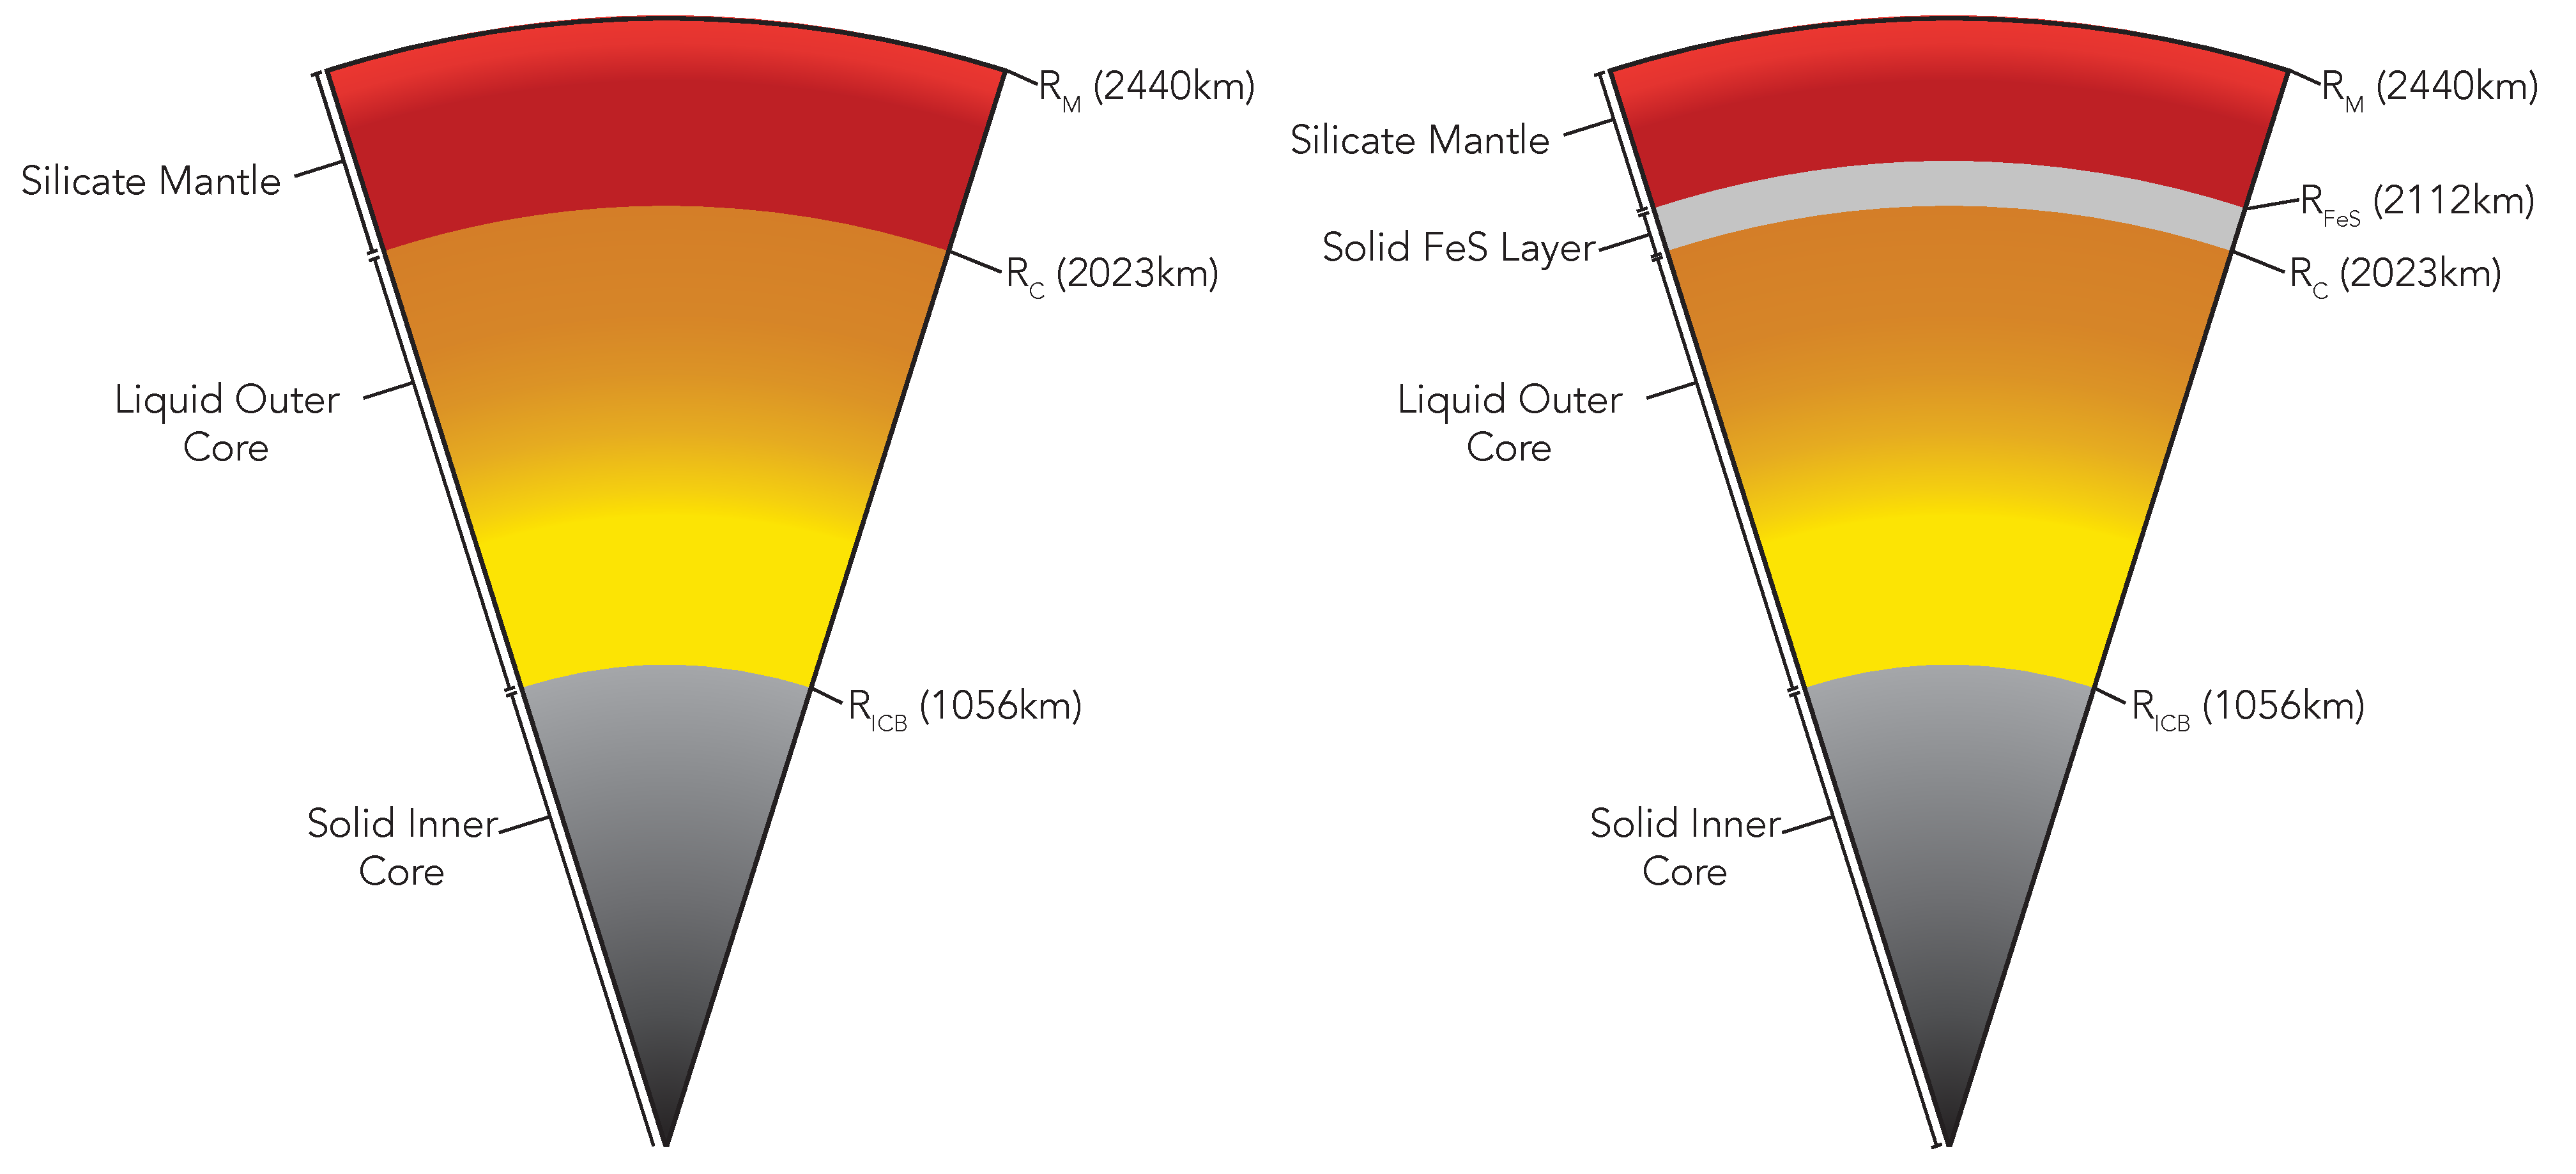
\includegraphics[width=\textwidth]{Chapter5/Figures/Structure.pdf}
        \caption{A schematic diagram of the models of Mercury's core presented in this chapter, without a FeS flotation layer (left) and with an FeS flotation layer (right).}
        \label{fig:FeSSchematic}
\end{figure}

All the simulations in this chapter were performed using the mMoSST numerical dynamo model. In these models the mantle was held fixed relative to the rotating planet frame, and the inner core was allowed to freely rotate due to magnetic and viscous torques. All fields (velocity, magnetic and co-density fields) were expanded to $L=100$ and $m=95$, and the inner core, fluid outer core and solid mantle layer have $75$, $80$ and $25$ radial gridpoints respectively. No hyperdiffusivities were used in any of the simulations in this chapter and the the non-axisymmetric inertial force is considered for all modes (see section \ref{chap:dynamotheory}).

In all cases, no-slip velocity boundary conditions and fixed temperature thermal boundary conditions were used at the inner core and core-mantle boundaries.

To get a range of local Rossby numbers we left most control parameters fixed and only varied the Rayleigh number. For all models $Ro=1\times10^{-5}$, $E=1\times10^{-5}$, and $q_k=5$, the Rayleigh number is varied between $5000$ and $35000$.

\section{Results}
The results of all of the simulations performed for this chapter are displayed in table \ref{tab:fesresults}. In this table $I_{\#}$ denotes a model with an insulating mantle (which corresponds to a model without a FeS flotation layer), and $C_{\#}$ denotes a model with a solid mantle layer which conducts electricity (which corresponds to a model with a FeS flotation layer). 

\begin{table}
\centering
\begin{tabular}{cllllllll}
\multicolumn{1}{l}{Model} & Ra    & Ro    & $\bar{\ell}_{u}$ & $Ro_{l}$ & $\tau_{dip}$ & $g_1^0 (\times 10^{3} \textrm{nT})$ & $g_2^0 (\times 10^{2} \textrm{nT})$ \\ \hline  %& Run & Subrun 
$I_{1}$                 & 8000  & 0.040 & 17.9             & 0.23     & 1.0          & 2.3                                 & -.961      &  \\                               %& 10  & 1      &  \\
$I_{2}$                 & 15000 & 0.064 & 19.9             & 0.41     & 0.45         & 2.0                                 & -2.18      &  \\                                %& 10  & 2      &  \\
$I_{3}$                 & 25000 & 0.090 & 20.4             & 0.58     & 0.46         & 3.5                                 & -1.03      &  \\                                %& 10  & 3      &  \\
$I_{4}$                 & 35000 & 0.11  & 20.4             & 0.73     & 0.30         & -1.4                                & -1.11      &  \\                               %& 10  & 4      &  \\
$C_{1}$                 & 8000  & 0.025 & 19.3             & 0.16     & 31.0         & 50                                  & -1.04      &  \\                               %& 11  & 1      &  \\
$C_{2}$                 & 15000 & 0.045 & 23.5             & 0.34     & 23.2         & 56                                  & -17.50      &  \\                                 %& 11  & 2      &  \\
$C_{3}$                 & 25000 & 0.068 & 24.8             & 0.54     & 16.4         & 63                                  & -4.73      &  \\                                 %& 11  & 3      &  \\
$C_{4}$                 & 35000 & 0.088 & 24.9             & 0.70     & 12.2         & 56                                  & -9.42      &                                   %& 11  & 4      & 
\end{tabular}
\caption{The results for all of the model simulations in this chapter. Here $I_{\#}$ denotes a model with an electrically insulating mantle, while $C_{\#}$ denotes a model with an electrically conducting mantle. The Rayleigh number is the only control parameter that changes between models, all other parameters are outlined in section \ref{sec:fesmodel}.}
\label{tab:fesresults}
\end{table}

\subsection{Validating the $\tau$--$Ro_{l}$ Scaling Law}
Before we discuss the applicability of our models to Mercury it is helpful to know whether the $Ro_l - \tau$ scaling law is accurate. In figure \ref{fig:tauscale} we have plotted the timescale of variation (equation \ref{eq:timescale}) of the dipole component of the magnetic field at the core mantle boundary ($\tau_{dip}$ in table \ref{tab:fesresults}) for models with a range of local Rossby numbers. In blue are the models which do not possess a solid FeS layer and in red are models which do. Both types of models follow the theoretical scaling law (equation \ref{eq:timescalescalinglaw}) very well. One noteworthy feature is that the addition of a solid FeS layer appears to reduce the timescale of variation of the dynamo by over an order of magnitude. This makes physical sense if we note that a solid electrically conducting layer at the top of the liquid outer core will strongly brake the fluid there due to the Lorentz force. This fluid is responsible for advecting the magnetic field close to the core-mantle boundary and causing the short timescale variations in it. If these flows are braked it follows that the timescale of variation of the magnetic field should also slow. Despite this, the timescale of variation with a conducting layer in place is still proportional to $Ro_l^{-0.88}$. 
\begin{figure}
	\centering
        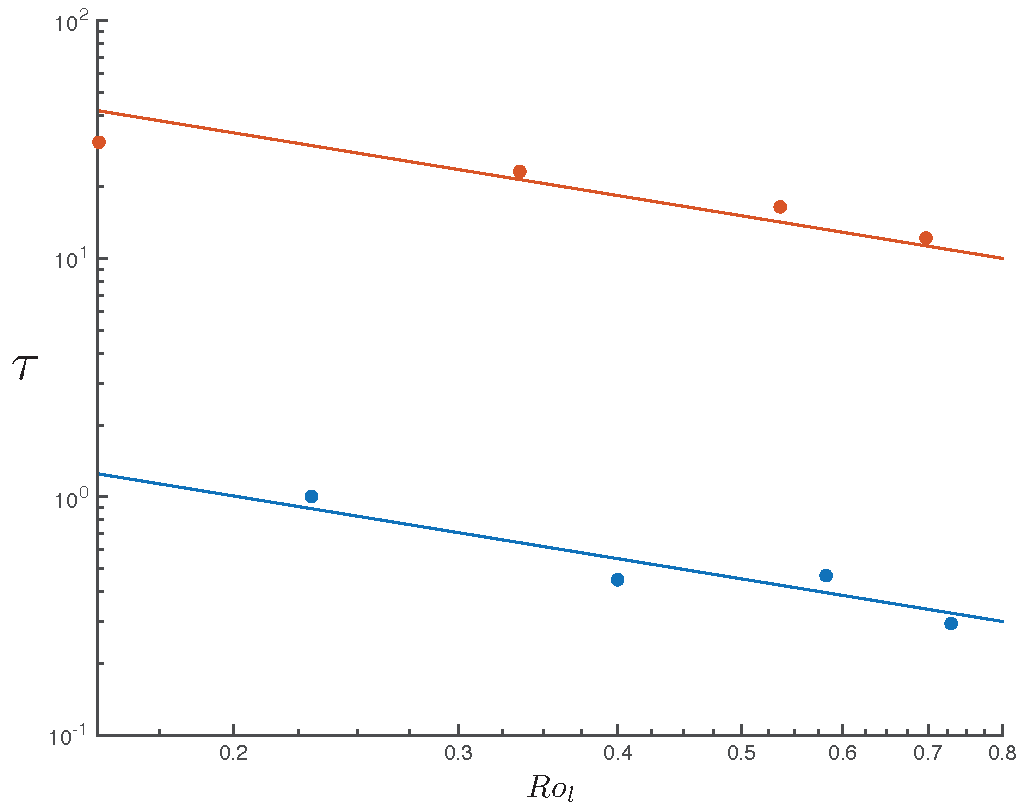
\includegraphics[width=.75\textwidth]{Chapter5/Figures/roltau.pdf}
        \caption{The timescale of core-mantle boundary dipole field variation as a function of local Rossby number for models with (red) and without (blue) a solid Fe-S mantle layer. The solid lines are best fit lines $\tau \propto  Ro_{l}^{-.875}$.}
        \label{fig:tauscale}
\end{figure}

\subsection{Magnetic Field}
\subsubsection{Gauss Coefficients and Locals Rossby Number}
The main observable we have to compare dynamo models of Mercury's magnetic field to the planet Mercury are the Gauss coefficients obtained from an analysis of the MESSENGER and Mariner 10 magnetometer data. Primarily, we we will compare the $g_1^0$ and $g_2^0$ Gauss coefficients which have been observed to be $190\pm14 \textrm{nT}$ and $74\pm \textrm{nT}$ respectively (see chapter \ref{chap:doublesnowstates} for more information on the observations of Mercury's magnetic field).

The strength of the $g_1^0$ and $g_2^0$ Gauss coefficients for each model is displayed in table \ref{tab:fesresults}. For the $I_{\#}$ models, the field is multipolar and small scale so the $g_1^0$ and $g_2^0$ components are quite small ($\mathcal{O}\left(10^{3}\right) nT$ and $\mathcal{O}\left(10^{2}\right) nT$ respectively). This is a key component of the model of \citet{christensen06}, the higher multipole are preferentially attenuated by the thick, stably stratified region above the convecting part of the core.

For the models which possess a solid, conducting mantle layer, the observed Gauss coefficients are far too strong to be compatible with Mercury's magnetic field. The $g_1^0$ coefficient is $\mathcal{O}\left(10^5\right) \textrm{nT}$ for all models, which is three orders of magnitude larger than the $g_1^0$ observed at Mercury. Also the $g_2^0$ component is two orders of magnitude too large and possesses the opposite sign as $g_1^0$. Both of these properties make the $g_2^0$ component incompatible with Mercury's observed magnetic field.

The addition of an electrically conducting mantle layer has a modest effect on the local Rossby number. In all models it appears as though the local Rossby number decreases slightly when a solid mantle layer is added (Table \ref{tab:fesresults}), however all remain above the critical value of $Ro_{l}\approx 0.12$. If the scaling of \citet{christensen06scaling} applies, we would predict a multipolar field for all models presented here. This decrease in local Rossby number stems from two competing effects, the addition of a FeS layer increases the predominant length scale of the velocity field ($\ell_u$) while decreasing the Rossby number ($Ro$, see table \ref{tab:fesresults}). Recall from section \ref{sec:rol} that the definition of the local Rossby number is
\begin{equation}
Ro_{l}=Ro\frac{\bar{\ell}_{u}}{\pi}.
\end{equation}
Because models with an FeS layer see their velocity, and hence their Rossby number decrease more than their length scale increases, the local Rossby number decreases when an FeS layer is added.

We can derive some insight into the large $g_1^0$ in the $C_\#$ models by examining the power spectrum (figure \ref{fig:powspec}). In this figure we see that the spectrum for a model without an FeS layer ($I_4$, red) has a range of less than an order of magnitude for the first 10 multipoles, with a peak at $L=3$. This is not surprising, as this model has a local Rossby number greater than $0.12$ and is run under the same parameters as the models that \citet{christensen06scaling} used to derive the local Rossby number.

The power spectrum for a model with a FeS flotation layer ($C_4$, blue) differs considerably from the spectrum of $I_4$. Here we see that the model is predominantly dipolar, as the $L=1$ component is over an order of magnitude stronger than the next strongest component ($L=5$).

The difference in power spectra that we observe in figure \ref{fig:powspec} provides a reason for the difference in $g_1^0$ that we see in table \ref{tab:fesresults}. The addition of an FeS layer has the effect of making the magnetic field much more dipolar than it would be otherwise. Since dipolar fields have $L=1$ they vary much more slowly than fields with higher $L$ so they are not efficiently screened by the solid conducting FeS layer. This results in a strong magnetic field at the surface and a $g_1^0$ component that does not match the observed $g_1^0$ of Mercury. 
\begin{figure}
	\centering
	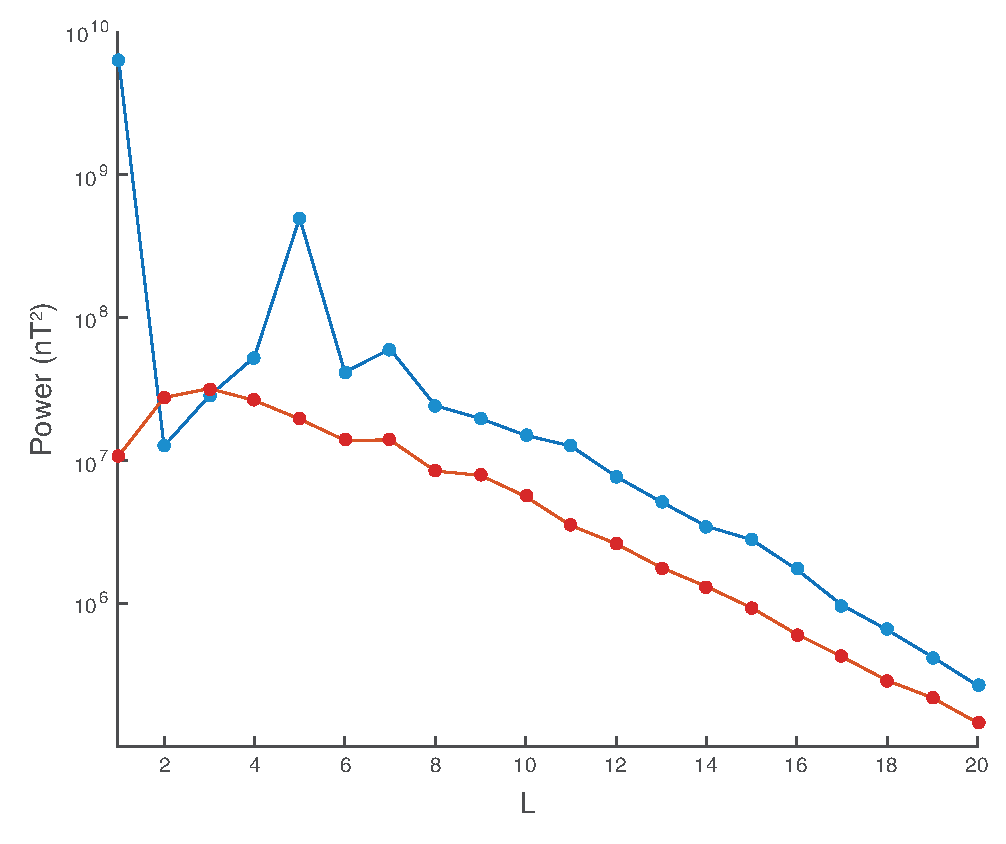
\includegraphics[width=.8\linewidth]{Chapter5/Figures/PowSpec.eps}

        \caption{The temporally averaged surface magnetic power spectrum for model $C_4$ (blue) and model $I_4$ (red). } 
        \label{fig:powspec}
\end{figure}

\subsubsection{Magnetic Field Morphology}
As we expected from the local Rossby number scaling laws, if we plot the radial magnetic field of models without a solid FeS mantle layer, the field morphology is highly non-dipolar and small scale (model $I_4$, figure \ref{fig:nofesbr}).
\begin{figure}
	\centering
        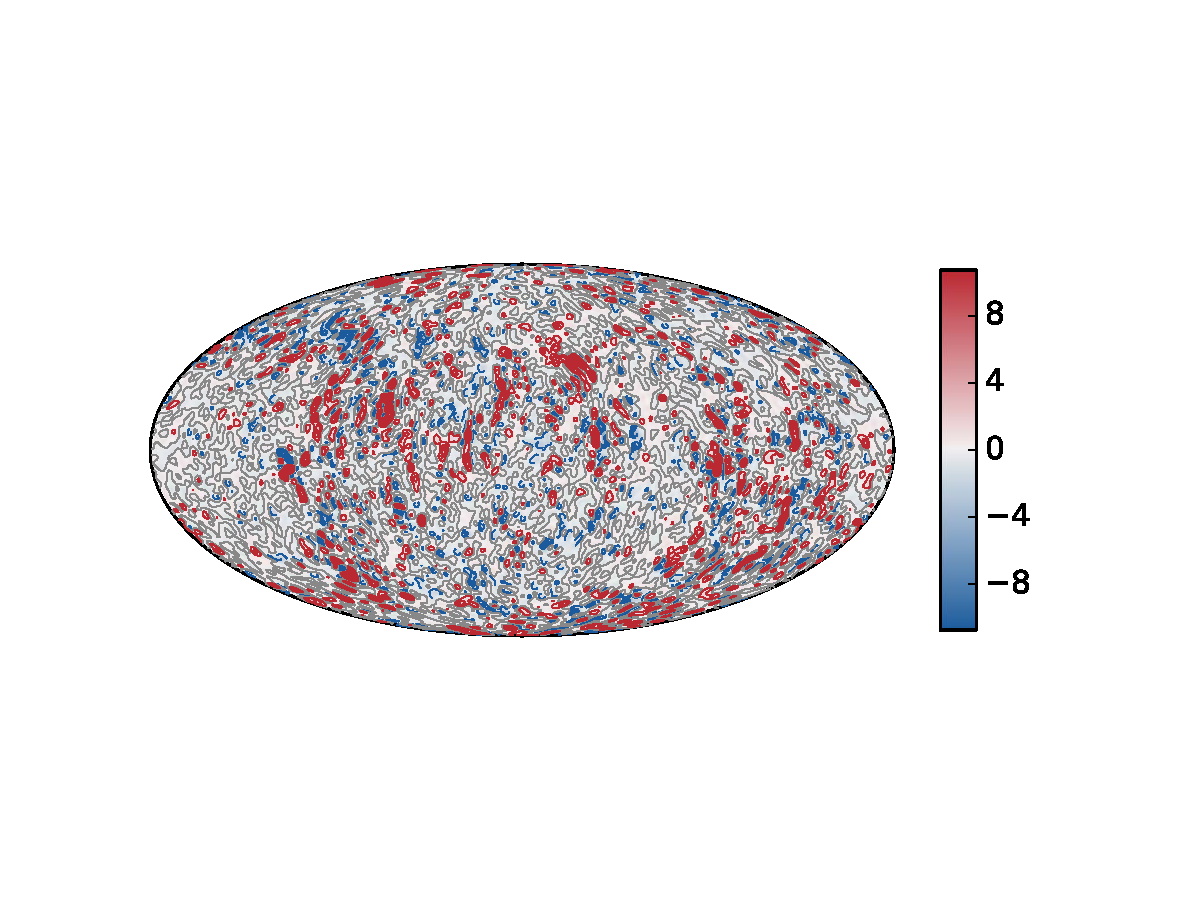
\includegraphics[width=.8\textwidth]{Chapter5/Figures/br10_004_1800_100.pdf} 
        \caption{A snapshot of the radial magnetic field at the core-mantle boundary for model $I_{4}$, units in this figure are non-dimensional.}
        \label{fig:nofesbr}
\end{figure}
The axisymmetric $\phi$ component of the magnetic field also displays very small scale magnetic field with no large scale field at all (model $I_{4}$, figure \ref{fig:nofesbax}). 
\begin{figure}
	\centering
	\begin{subfigure}{.4\textwidth}
		\centering
	        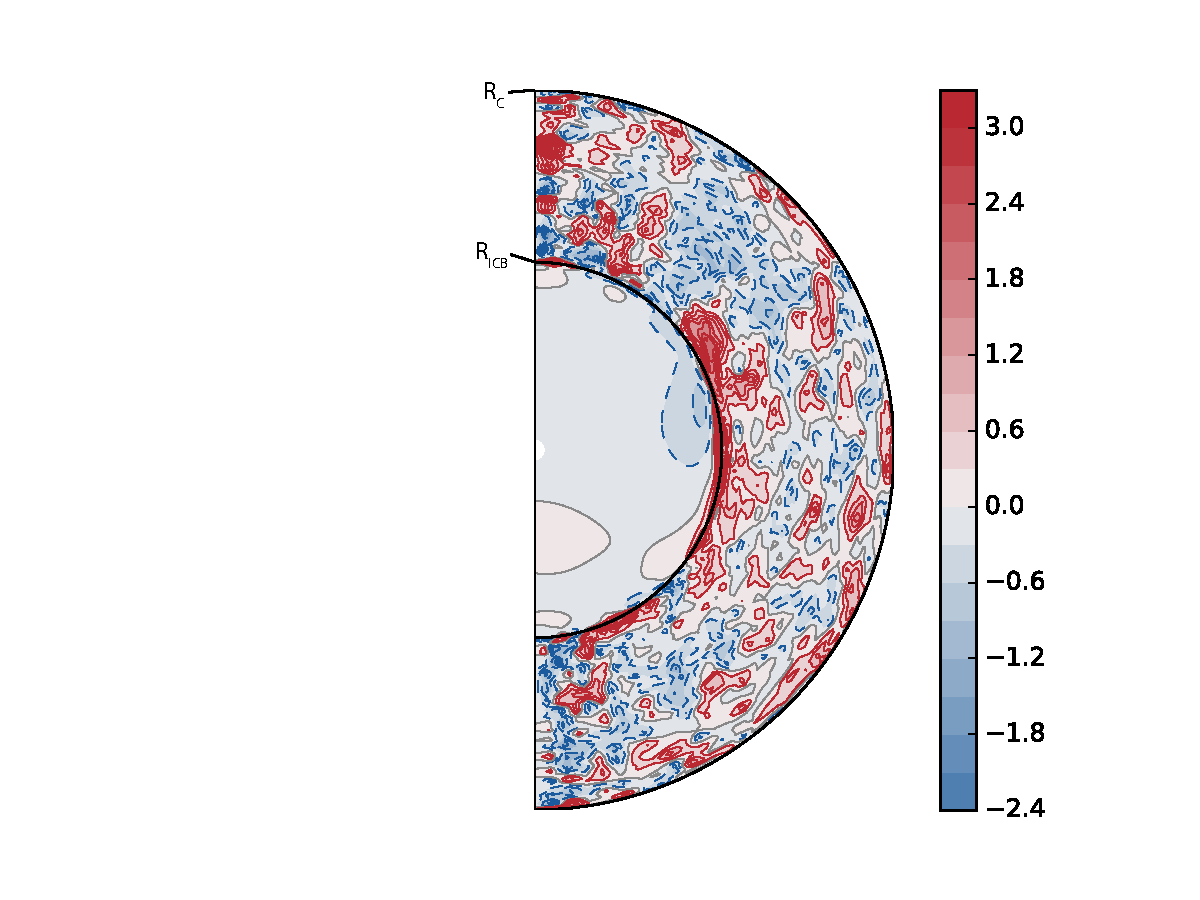
\includegraphics[width=\linewidth]{Chapter5/Figures/btor10_004_1800.pdf}
     		
		\caption{\label{fig:nofesbax}}
        \end{subfigure}%
        \begin{subfigure}{.4\textwidth}
	        \centering
	        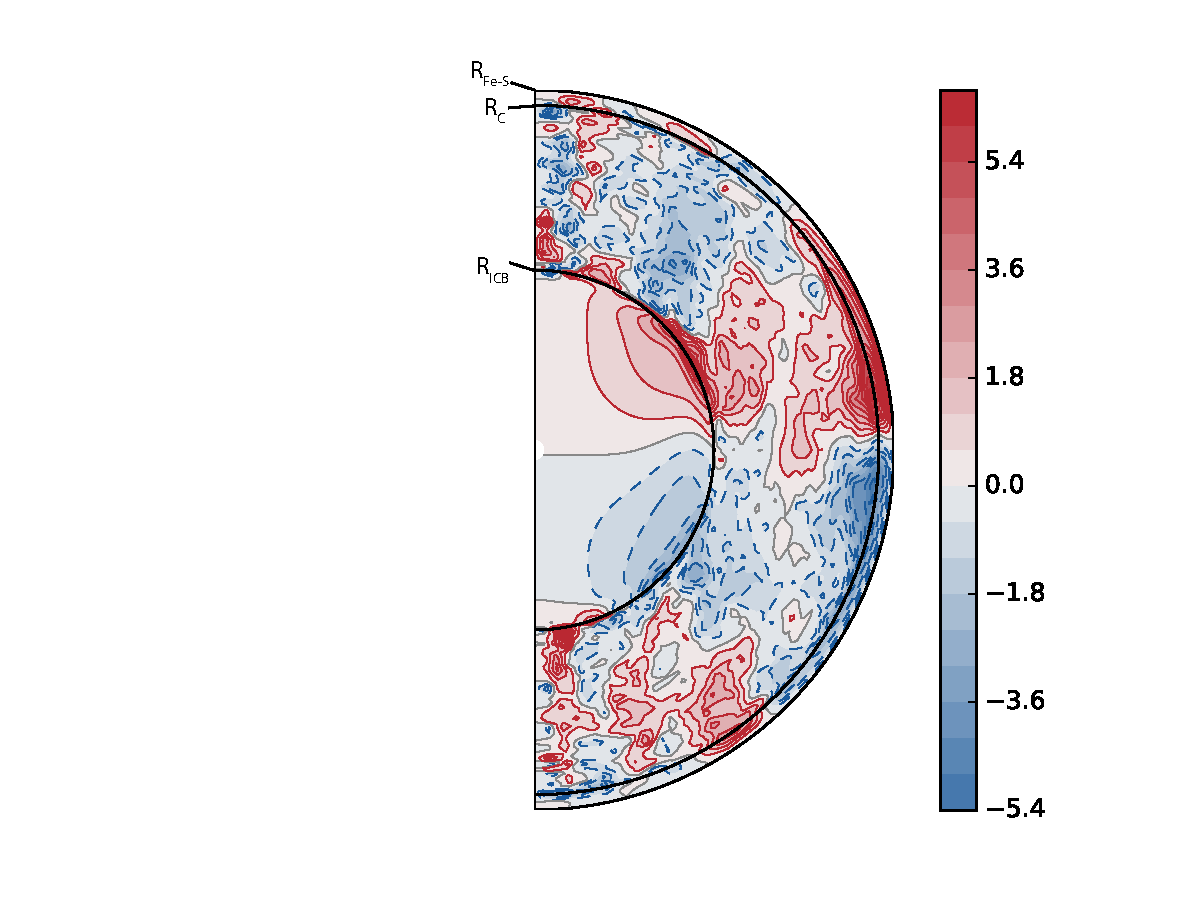
\includegraphics[width=\linewidth]{Chapter5/Figures/btor11_004_1631.pdf}
	       
	        \caption{ \label{fig:fesbax}}
        \end{subfigure}
        \caption{Snapshots of the axisymmetric $\phi$ component of the magnetic field within the core for model $I_{4}$ (\subref{fig:nofesbax}) and model $C_{4}$ (\subref{fig:fesbax}). The region nearest the centre of the semicircle in both figures is the inner core, followed by the fluid outer core (moving outwards) followed by the conducting mantle layer in model $C_4$. Units in these figures are non-dimensional.}
\end{figure}
If we examine the axisymmetric $\phi$ component of the field within the core and conducting layer for a model with an FeS mantle layer (figure \ref{fig:fesbax}), we find very similar results to what we saw in chapter \ref{chap:superearth}. Near the core-mantle boundary very strong axisymmetric $\phi$ field is generated by the shear between the stationary, solid mantle and the strong, large scale zonal flows that exist within the fluid outer core (figure \ref{fig:fesutor})
\begin{figure}
	\centering
        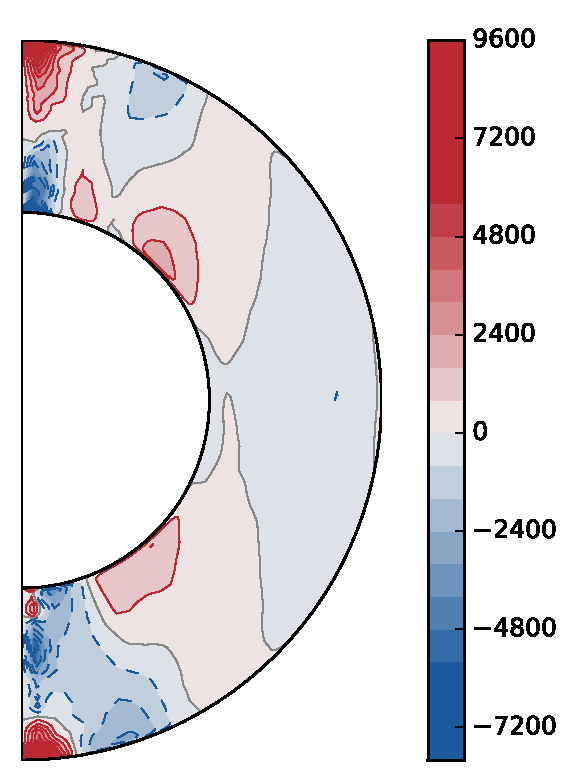
\includegraphics[width=.4\textwidth]{Chapter5/Figures/utor11_004_1500-1630.pdf} 
        \caption{The time average of the axisymmetric $\phi$ component of velocity for model $C_4$.}
        \label{fig:fesutor}
\end{figure}
. There is a stark difference between the axisymmetric $\phi$ field in the case without a solid conducting layer (figure \ref{fig:nofesbax}) and the models with a conducting layer (figure \ref{fig:fesbax}). The magnetic shear at the core-mantle boundary has the effect of dramatically increasing the length scale of the axisymmetric toroidal magnetic field. It also organises the axisymmetric $\phi$ component of the field into a pattern more commonly seen in models with a much lower local Rossby numbers, which generate dipolar magnetic fields (e.g. figure \ref{fig:maggen}a).

This shear of the magnetic field is also evident in plots of the $\phi$ component of the magnetic field at the core-mantle boundary. In figure \ref{fig:nofesbph} we see that without a solid, electrically conducting layer the field is very small scale and disorganised. Once an electrically conducting solid mantle layer is added (figure \ref{fig:fesbph}) the large scale shear imposed by the zonal flows dramatically increases the length scale of the $\phi$ component of the field.
\begin{figure}
	\centering
	\begin{subfigure}{.8\textwidth}
		\centering
	        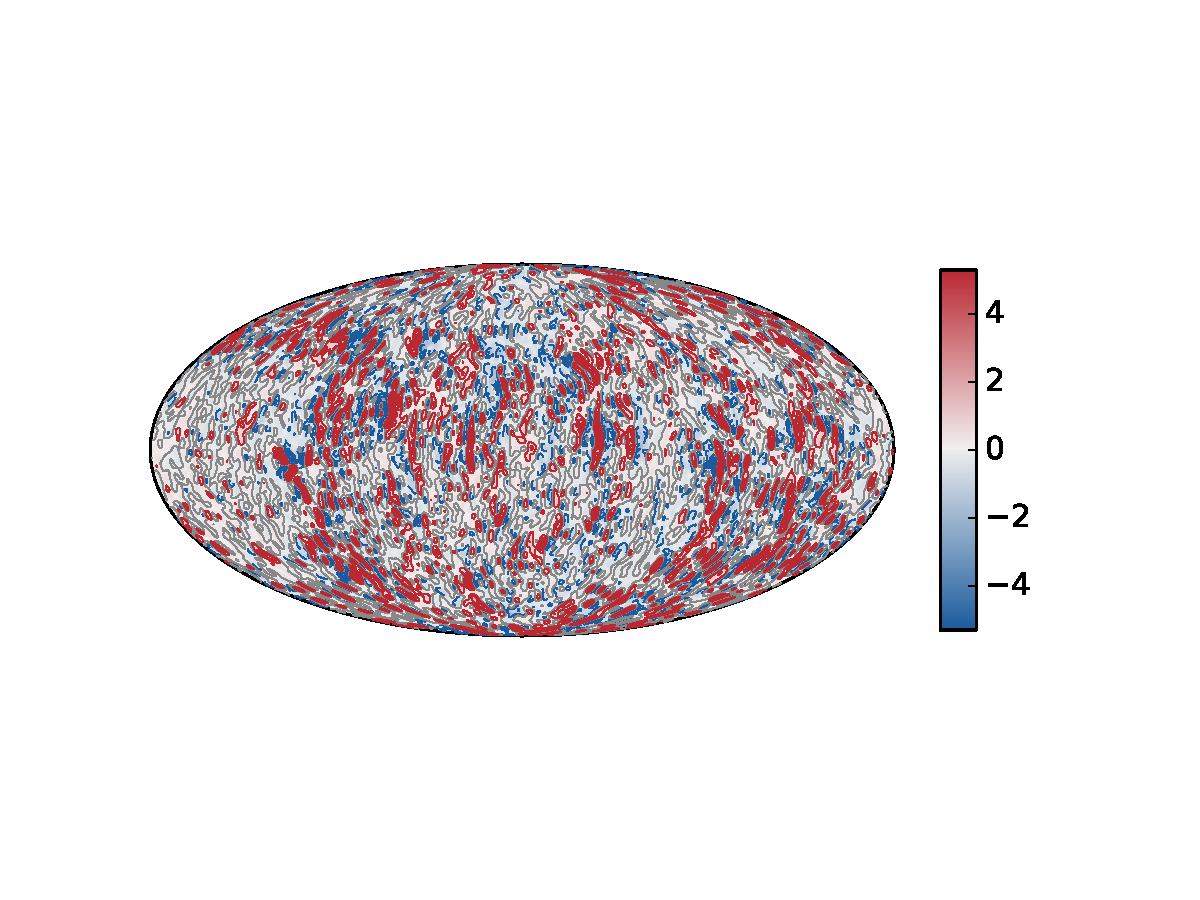
\includegraphics[width=\linewidth]{Chapter5/Figures/bph10_004_1800_100.pdf}
     		
		\caption{\label{fig:nofesbph}}
        \end{subfigure}
        
        \begin{subfigure}{.8\textwidth}
	        \centering
	        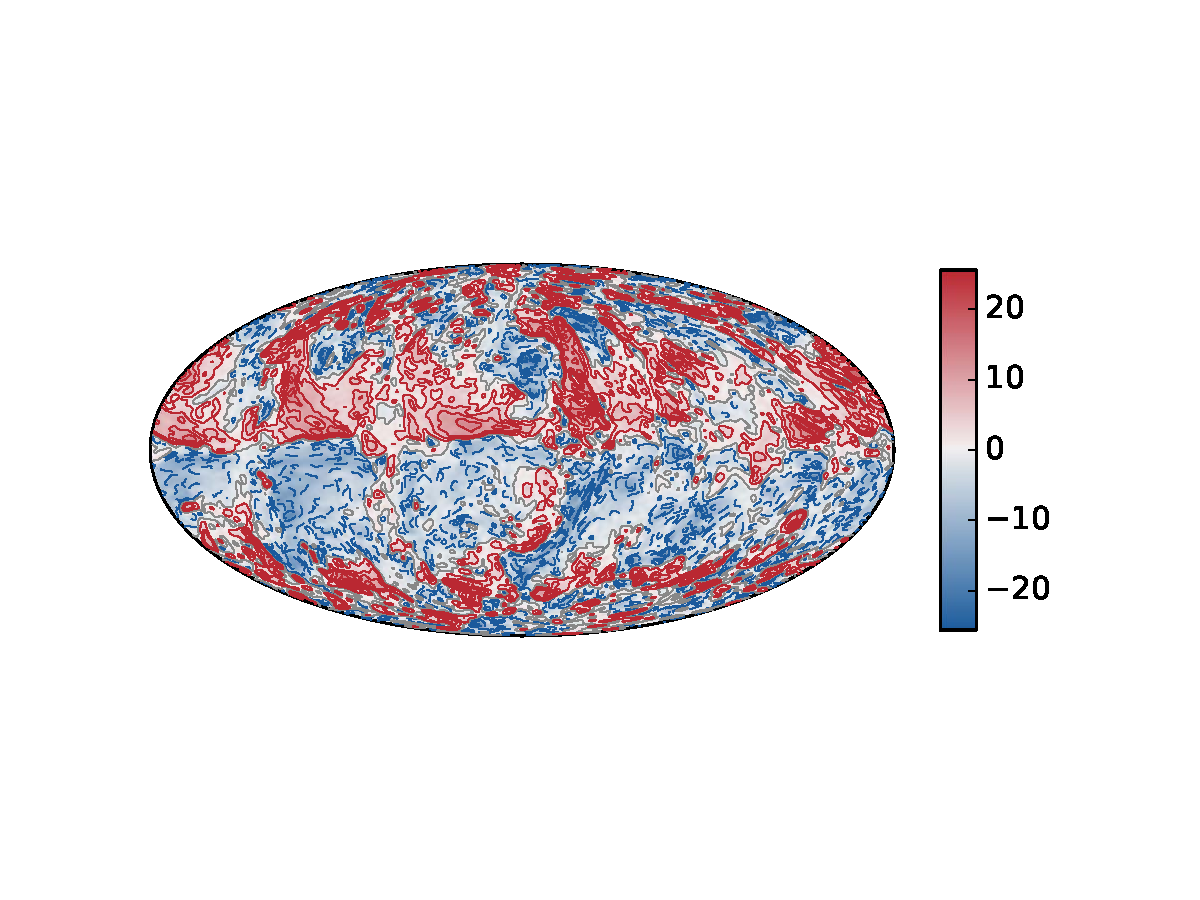
\includegraphics[width=\linewidth]{Chapter5/Figures/bph11_004_1631_100.pdf}
	       
	        \caption{ \label{fig:fesbph}}
        \end{subfigure}
        \caption{Snapshots of the $\phi$ component of the magnetic field at the core-mantle boundary for a model without an FeS layer (\subref{fig:nofesbph}) and with an FeS layer (\subref{fig:fesbph}). Units in these figures are non-dimensional and are from models $I_4$ and $C_4$.} 
        \label{fig:bph}
\end{figure}

This large scale toroidal magnetic field generates a radial magnetic field which is also large scale, and predominantly dipolar (figure \ref{fig:fesbrcmb}). This is a completely different magnetic field morphology compared to the insulating mantle model at the same parameters (figure \ref{fig:fesbrcmb}).
\begin{figure}
	\centering
	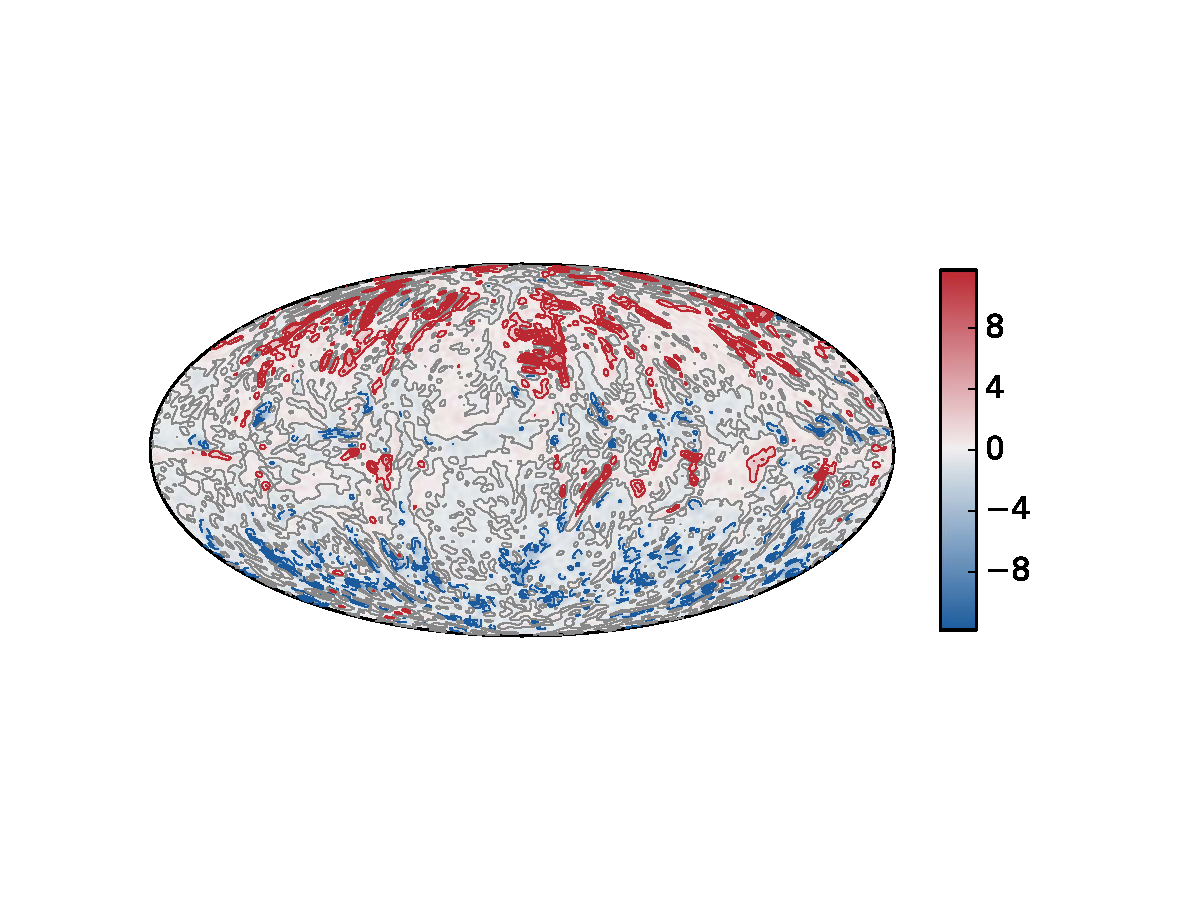
\includegraphics[width=.8\linewidth]{Chapter5/Figures/br11_004_1631_100.pdf}	
	\caption{A snapshot of the radial component of the magnetic field at the core-mantle boundary for model $C_4$. Units in this figure are non-dimensional.}
	\label{fig:fesbrcmb}
\end{figure}
As we discussed in chapter \ref{chap:superearth}, if there is an electrically conducting mantle layer present in the model the radial component of the magnetic field at the core-mantle boundary is modified before it is observed at the surface. The conducting mantle layer will attenuate the field by a factor of $e^{-d\sqrt{\omega/(2 \eta)}}$ (refer to chapter \ref{chap:superearth} for a discussion of this factor). In figure \ref{fig:fesbrddp} we plot the radial component of the magnetic field above the conducting FeS layer and see that the strength of the magnetic field has been reduced somewhat and the length scales have increased.
\begin{figure}
	\centering
	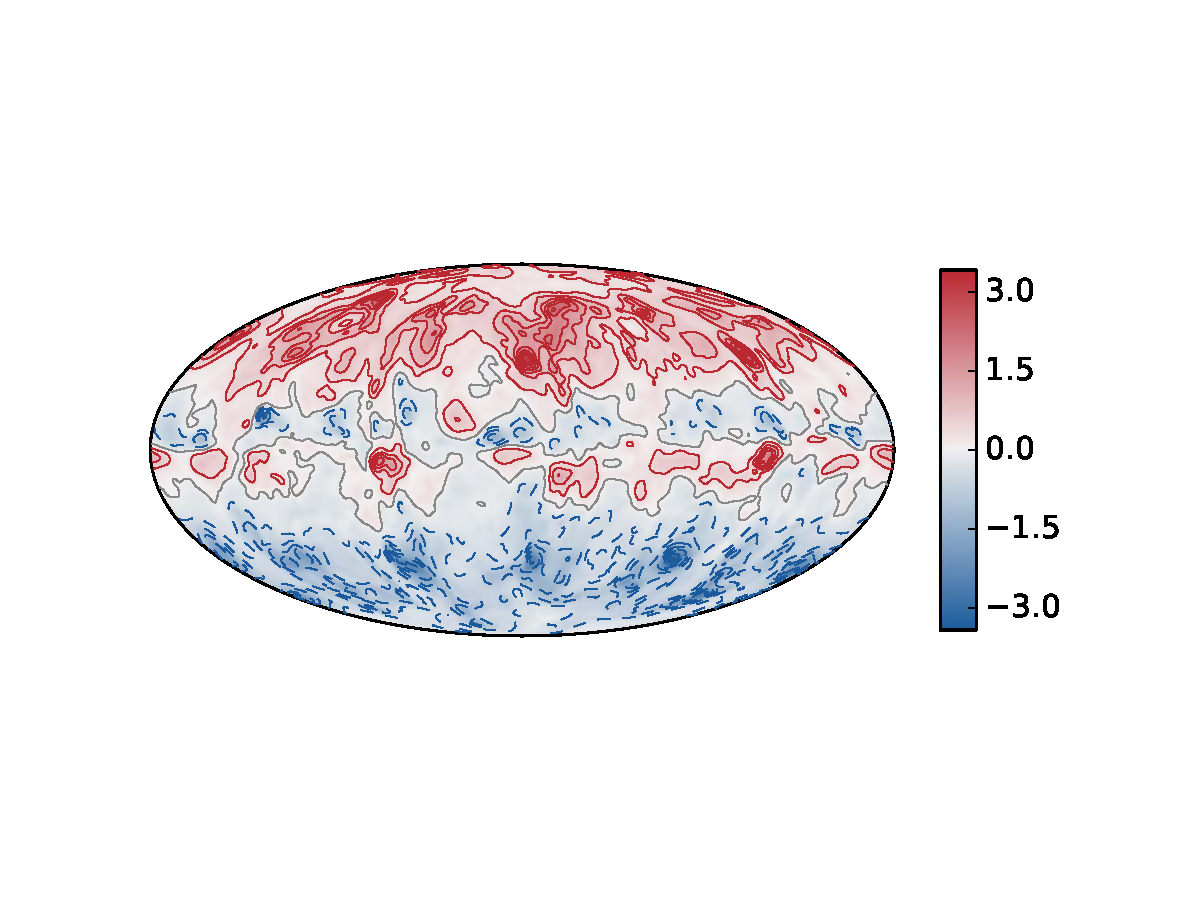
\includegraphics[width=.8\linewidth]{Chapter5/Figures/br11_004_1631_104.pdf}
	\caption{A snapshot of the radial component of the magnetic field at the top of the electrically conducting mantle for model $C_4$. Units in this figure are non-dimensional.}
        \label{fig:fesbrddp}
\end{figure}

Finally, in figure \ref{fig:fessurf} we plot the dimensional radial magnetic field at the surface for model $C_4$. Here it is obvious that this model does not match Mercury's magnetic field at all. The surface fields we observe in figure \ref{fig:fessurf} are several orders of magnitude too large to be consistent with Mercury's magnetic field. Also, we can see that the magnetic equator and the planetary equator appear coincident which is also inconsistent with the observed $400\textrm{km}$ northward shift of Mercury's magnetic equator (figure \ref{fig:Mercurybr}).
\begin{figure}
	\centering
        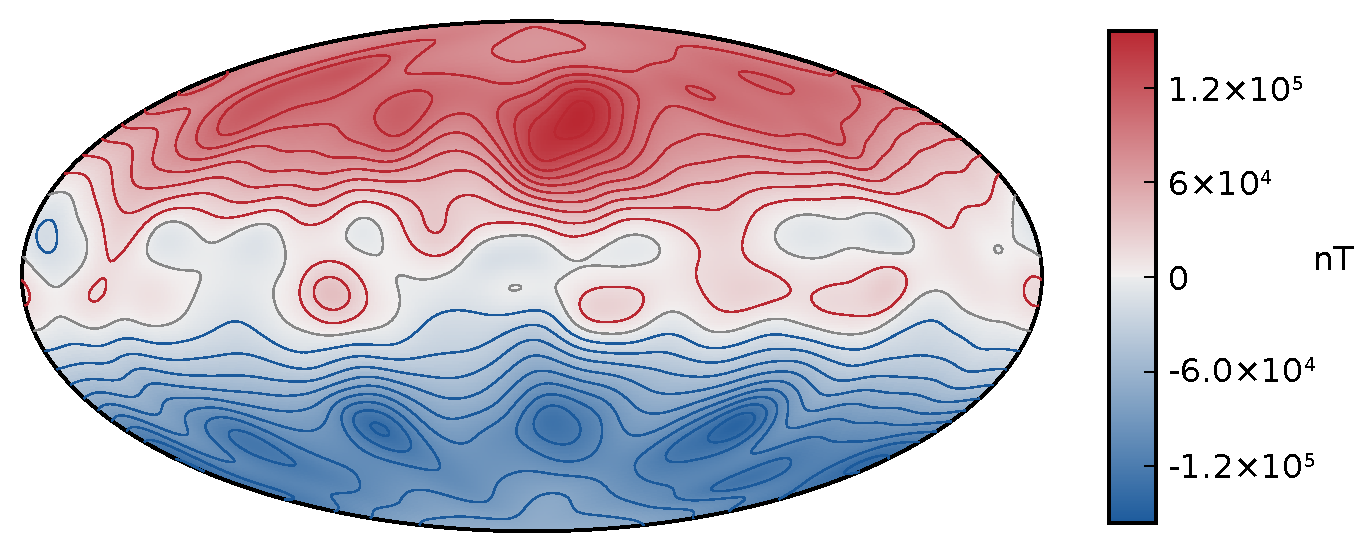
\includegraphics[width=\linewidth]{Chapter5/Figures/br11_004_1631_surf.pdf} 
        \caption{A snapshot of the surface radial magnetic field for model $C_4$ in dimensional units.}
        \label{fig:fessurf}
\end{figure}

In the models presented here we have found that the addition of a solid FeS layer causes the field to become much more dipolar. The reason for this is because of the large scale axisymmetric $\phi$ field sheared out by the zonal flows present in our models. The large scale axisymmetric $\phi$ field that is sheared by these flows is then the seed field for the poloidal field. As large scale seed field tends to create large scale resultant field, the poloidal field from our models is strong and predominantly dipolar.

\section{Conclusion}
We have tested the consequences of a solid, conducting FeS layer on magnetic field generation in Mercury. Models of Mercury's interior have allowed for a deep, dense layer in Mercury's mantle which some studies \citep{smith2012, hauck2013} suggested could explain Mercury's weak axial dipole via the screening effect \citep{christensen06}. We found that when all the consequences of a solid, electrically conducting layer are considered, the addition of a solid FeS layer causes the dynamo to change from generating a multipolar magnetic field to a dipolar field. This strong dipolar field does not vary quickly enough to be effectively screened by the mantle layer, and a magnetic field several orders of magnitude too large to be consistent with Mercury's field is observed at the planetary surface.

This has interesting implications for the scaling laws of \citet{christensen06scaling}. All the models which have a solid conducting mantle layer have a local Rossby number greater than $0.12$, which implies that they should generate a predominantly non-dipolar magnetic field. As we found in this study, while the $\tau-Ro_l$ scaling law appears to apply once an FeS layer is added (figure \ref{fig:tauscale}) the transition point in local Rossby number is not valid in this new geometry. Furthermore, local Rossby number appears to decrease once an electrically conducting mantle layer is added (table \ref{tab:fesresults}) meaning that the scaling law which relates the control parameters to the local Rossby number (equation \ref{eq:rolscaling}) may need to be modified. 

One unresolved question from this study is whether there exists a parameter regime in which the local Rossby number is high enough for a dynamo model with a solid FeS layer to display a multipolar magnetic field. Currently the field is predominantly dipolar because the dynamo is seeded with large scale, dipolar toroidal magnetic field from the shear created between the solid mantle and the zonal flows in the fluid outer core. At high enough buoyancy fluxes (Rossby numbers) the homogenisation of magnetic flux due to convection may outstrip the ability of zonal flows to generate large scale toroidal field and a multipolar field could result. As we are unable to run at a local Rossby number that is realistic for Mercury, we do not currently know whether this possible transition is above the local Rossby number that we expect for Mercury ($\mathcal{O}\left(10^1\right)$).
%
%It would seem as though the results that we have found in this chapter contradict the results of chapter \ref{chap:superearth}. In chapter \ref{chap:superearth} we found that the addition of a solid conducting mantle layer made the dynamo less axisymmetric, while in this chapter we found that the addition of a solid conducting mantle layer made the dynamo more dipolar and more axisymmetric. 
%
%A key difference between these two chapters is the parameter regime of the dynamo. In chapter \ref{chap:superearth} the dynamo was chosen to be in a parameter regime of $Ro_{l}<0.12$, meaning that in the absence of a solid conducting mantle layer the dynamo would generate large scale, dipolar fields. In this chapter the parameter regime was chosen so that $Ro_{l}>0.12$ meaning that the generated magnetic field is much smaller scale and non-dipolar.
%
%Common to the models of this section and chapter \ref{chap:superearth} are large scale axisymmetric zonal flows (for example \ref{fig:fesutor}). These flows are caused by a combination of thermal winds and Reynolds stresses and are a common feature of rotating convective systems. In the context of dynamos, they have been studied in detail by \citet{aubert2005zonal}. As we discussed in chapter \ref{chap:superearth}, these zonal flow provide source of shear at the CMB for models with an electrically conducting mantle layer. Poloidal field lines are frozen into the solid immobile mantle and the strong, axisymmetric zonal flows causing a large magnetic shear at the boundary. The effects of this shear are obvious in plots of the axisymmetric toroidal field for  these models (figures \ref{fig:toroidal} and \ref{fig:fesbax}). In these figures large regions of axisymmetric $\phi$ magnetic field are sheared out at the core-mantle boundary by the zonal flows present in both models. 
%
%In the models 

%We can gain some insight into why the models with solid FeS layers generate large scale magnetic fields by considering poloidal magnetic field generation with the Bullard-Gellman formalism (see Appendix \ref{chap:appendix1}) in the scenario where the core has already been seeded with the large scale toroidal field pattern we see in figure \ref{fig:fesbax}. For this scenario we focus on the generation of poloidal field by velocities acting on toroidal fields. These correspond to 
%\begin{equation}
%P_\alpha T_\beta P_\gamma
%\end{equation}
%and
%\begin{equation}
%T_\alpha T_\beta P_\gamma.
%\end{equation}
%Recall that $P$ stands for poloidal and $T$ stands for toroidal, and $\alpha$, $\beta$ and $\gamma$ refer to the velocity field, the seed magnetic field and the resultant magnetic field respectively. We showed in appendix \ref{chap:appendix1} that the latter of these is always zero, but $P_\alpha T_\beta P_\gamma$ requires some analysis.
%
%We see that the toroidal field pattern in figure \ref{fig:fesbph} is predominantly dipolar so we will assign $\beta=1$, $m_\beta=0$ and look at which modes of velocity and magnetic field can make this integral non-zero. The $P_\alpha T_\beta P_\gamma$ integral is an Elsasser type integral, which has its selection rules printed in appendix \ref{chap:appendix1}. For our purposes we are mainly interested in two of these:
%\begin{quote}
%An Elsasser type integral is zero unless:
%\begin{itemize}
%\item $\alpha, \beta, \gamma$ can form the sides of a triangle. This is equivalent to satisfying the triangle inequality: $\left|\alpha-\beta\right|<\gamma<\alpha+\beta$.
%\item One or more of $m_\alpha \pm m_\beta \pm m_\gamma$ is zero.
%\end{itemize}
%\end{quote}
%These two rules constrain the magnitude of $m$ and $L$ of the resultant magnetic field $\gamma$ and velocity field $\alpha$. If $\beta=1$ and $m_\beta=0$ this means that
%\begin{equation}
%\left|\alpha-1\right|<\gamma<\alpha+1
%\end{equation}
%and one or more of 
%\begin{equation}
%m_\alpha \pm  m_\gamma  = \pm1.
%\end{equation}
%These equations show that $\alpha \approx \gamma$ and $m_\alpha \approx m_\gamma$